\chapter{Localization of quantum walks}
\label{ch:quantum}

\section{A walker that does not forget}

This book opened with a walk. Chapter~\ref{ch:search} put a surfer on a network,
let it step from node to node, and found that the mere act of walking manufactures
preferential attachment: a page reached by many routes is reached often, so it
grows. Everything since has been an elaboration of that idea --- other local rules,
other systems, but always a newcomer that acts on what is near it. It is fitting to
close by putting a walker back on the networks those rules built, and asking what
it finds. The answer turns out to say something the earlier chapters could not say
about the rules themselves.

The walker of Chapter~\ref{ch:search} was classical, and classical walkers forget.
On any connected network a random walk settles, after long enough, into the same
stationary distribution --- each node visited in proportion to its degree, $v_i =
k_i/2m$ --- and it settles there no matter where it started. That is precisely what
made the chapter work: the visiting probability could be treated as a property of
the node, not of the walk's history. It is also a kind of blindness. The stationary
distribution of a random walk knows the degree sequence and nothing else. Two
networks with the same degrees --- one grown by triadic closure, one wired at random
--- look identical to it. A classical walk cannot tell us which rule built the
network it is walking on.

A \emph{quantum} walker does not forget. Replace the diffusion equation with the
Schr\"odinger equation and the evolution becomes unitary: probability is shuffled
between nodes without ever being dissipated, amplitudes interfere, and there is no
stationary distribution to relax into \citep{farhi1998,kempe2003,mulken2011}. Where
a classical walk erases its initial condition, a quantum walk carries it forever.
And because it carries it forever, it can be asked a question a classical walk
cannot answer: \emph{how much of the network did the walker ever reach?}

That question has a sharp answer, and the answer, it turns out, is a fingerprint of
the growth rule. This chapter is about measuring it.

The immediate provocation is a paper of \citet{boettcher2025localization}, who put
continuous-time quantum walks on networks built by recursively attaching triangles
and found the walker trapped: confined for all time to a handful of nodes around
where it started. They found the same in two other highly clustered constructions
and concluded that local clustering induces localization. Their networks are close
cousins of the pseudofractal web of Chapters~\ref{ch:communities}
and~\ref{ch:motifs}, and their triangles are the triangles of
Chapter~\ref{ch:friends}, so the result reads like a statement about this book. It
nearly is. What the measurements below show is that clustering is the wrong
variable --- that it is a correlate of the effect and not its cause --- and that the
right variable is one this book already has a name for.

\section{The measure of confinement}

Fix a network of $n$ nodes with adjacency matrix $A$, degrees $k_i$, and let $D$ be
the diagonal matrix of degrees. The walker's state is a complex amplitude on every
node, $\ket{\psi(t)}$, normalized so that $\braket{\psi|\psi}=1$, and it evolves by
the Schr\"odinger equation
\begin{equation}
  \frac{\mathrm{d}}{\mathrm{d}t}\ket{\psi(t)} = -\mathrm{i}\,H\ket{\psi(t)},
  \qquad
  H = D^{-1/2}\big(D-A\big)D^{-1/2},
  \label{eq:qw-schrodinger}
\end{equation}
whose solution is $\ket{\psi(t)}=e^{-\mathrm{i}Ht}\ket{\psi(0)}$. The generator $H$
is the symmetric normalized Laplacian, the standard choice for walks on networks
\citep{faccin2013,boettcher2025localization} and the one whose \emph{ground state}
reproduces the classical stationary distribution, so that the quantum and classical
walkers agree about where a walker at rest should be found and disagree only about
motion. The probability of finding a walker that started at node $j$ on node $i$ at
time $t$ is
\begin{equation}
  \pi_{ij}(t) = \big|\bra{i}e^{-\mathrm{i}Ht}\ket{j}\big|^2 .
  \label{eq:qw-prob}
\end{equation}

How spread out is that distribution? The standard instrument, borrowed from the
theory of electrons in disordered solids \citep{thouless1974,wegner1980}, is the
\emph{inverse participation ratio}
\begin{equation}
  \mathrm{IPR}_j(t) = \sum_{i=1}^{n} \pi_{ij}(t)^2 ,
  \label{eq:qw-ipr}
\end{equation}
and it is easiest to read through its reciprocal. If the walker's probability is
spread evenly over $\ell$ nodes and is zero on the rest, then each of those $\ell$
nodes carries $\pi=1/\ell$ and Eq.~\eqref{eq:qw-ipr} gives
$\mathrm{IPR}=\ell\cdot(1/\ell)^2 = 1/\ell$. So
\begin{equation}
  \ell \;=\; \frac{1}{\mathrm{IPR}}
  \label{eq:qw-ell}
\end{equation}
is the \emph{localization volume}: the effective number of nodes the walker
occupies, counted in a way that does not care how the probability is distributed
among them. Its two extremes bracket everything that follows. A walker pinned to a
single node has $\ell=1$. A walker spread uniformly over the whole network has
$\ell=n$.

That contrast is the whole measurement, and it is a statement about how $\ell$
depends on $n$. A walk is \emph{delocalized} if $\ell$ grows in proportion to the
network --- the walker occupies a fixed \emph{fraction} of a growing system, so it
explores everything. It is \emph{localized} if $\ell$ approaches a constant --- the
walker occupies a fixed \emph{number} of nodes however large the network becomes,
so the fraction it explores goes to zero. There is no need for a threshold value of
the IPR to separate the two cases, which is fortunate, because no natural one
exists \citep{boettcher2025localization}. One only has to grow the network and see
whether $\ell$ moves.

Because the evolution is unitary, $\mathrm{IPR}_j(t)$ never settles down; it
oscillates forever. The quantity to compare across networks is therefore its
long-time mean, $\overline{\mathrm{IPR}_j} = \lim_{T\to\infty}T^{-1}\int_0^T
\mathrm{IPR}_j(t)\,\mathrm{d}t$, which does converge, and which can be written in
closed form. The form is worth seeing once, because it identifies what a network
must supply in order to trap a walker.

\begin{calculation}{the long-time mean, and what makes it large}
Expand in the eigenbasis of $H$, writing $He_m = \lambda_m e_m$. Then
\begin{equation}
  \pi_{ij}(t) = \sum_m A_m^{ij} + \sum_{m<\,n} B_{mn}^{ij}
               \cos\!\big[(\lambda_m-\lambda_n)t\big],
  \label{eq:qw-pi-expand}
\end{equation}
with $A_m^{ij}=|\braket{i|e_m}\braket{e_m|j}|^2$ and
$B_{mn}^{ij}=2\braket{i|e_m}\braket{e_m|j}\braket{j|e_n}\braket{e_n|i}$. Averaging
over time kills every oscillating term whose frequency is nonzero, so
\begin{equation}
  \bar\pi_{ij} = \sum_m A_m^{ij}
    + \sum_{\substack{m<n\\ \lambda_m=\lambda_n}} B_{mn}^{ij} .
  \label{eq:qw-pibar}
\end{equation}
Squaring Eq.~\eqref{eq:qw-pi-expand} before averaging keeps more: a product of two
cosines survives whenever the four eigenvalues involved satisfy
$\lambda_m-\lambda_n=\lambda_s-\lambda_r$, which happens for degenerate pairs and
for \emph{quartets} with matching spacings \citep{boettcher2025localization}.

The lesson does not depend on writing the quartet sums out. A large long-time IPR
requires a network whose Hamiltonian has \emph{degenerate eigenvalues}, or at least
many coincident gaps, because those are the terms that do not average away.
Degeneracy, in turn, is what symmetry produces. So a rule that builds symmetric
local structure --- the same small configuration, over and over --- is a rule that
manufactures exactly the spectral coincidences the walker needs in order to stay
put. This is the thread that Section~\ref{sec:qw-twins} pulls hardest.
\end{calculation}

Everything reported below is a numerical time-average of Eq.~\eqref{eq:qw-ipr} over
a late window, $t\in[400,800]$, sampled at $240$ points, for $24$ start nodes $j$
drawn at random from each network and averaged over them; the walk itself is
computed exactly, by diagonalizing $H$ and phasing its eigenbasis, so the only
approximation is the finite window. Widening the window to $t\in[1600,3200]$ moves
no value reported here by more than about seven percent, and reverses none of the
comparisons. Each stochastic rule is grown ten times at each size. The rules are
the generators of Chapters~\ref{ch:communities} to~\ref{ch:bubbles}, imported
unchanged, so that the networks walked on here are the same networks those chapters
fitted.

\section{Every local rule traps the walker}
\label{sec:qw-flat}

Figure~\ref{fig:qw-density} shows the phenomenon before any averaging. On the left,
a walker started on a network grown by $BB(n,1)$ --- lay a new node across a random
link, closing a triangle --- and left to run. It does not go anywhere. The
probability sloshes back and forth among a few nodes near the start, and the rest of
the network --- three decades fainter --- never fills in, for as long as one cares to
watch. On the right, the same
walker on a ring of the same size, spreading ballistically outward as one would
expect of a wave.

\begin{figure}[t]
\centering
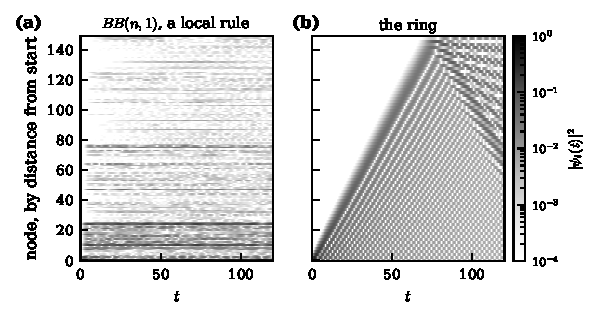
\includegraphics[width=\linewidth]{figs/fig-qw-density.pdf}
\caption{\textbf{A walker that stays, and a walker that goes.} Probability
$|\psi_i(t)|^2$ against node and time, for a walk started on a single node, with
nodes ordered by their distance from that node so that spreading appears as
widening. (a) On $BB(n,1)$, $n=150$, the walker never leaves a neighborhood of its
starting point. (b) On a ring of $150$ nodes it moves away at constant speed and
wraps around. Darker is more probable; the color scale is logarithmic, because a
linear one that resolves the trapped walker leaves the ring almost blank.}
\label{fig:qw-density}
\end{figure}

\begin{center}
\footnotesize\setlength{\tabcolsep}{3pt}
\begin{tabular}{llrrrrrrr}
\hline
 & & & & \multicolumn{4}{c}{$\ell=1/\overline{\mathrm{IPR}}$} & \\
rule & motif & $\langle c\rangle$ & $\langle k\rangle$ & $100$ & $200$ & $400$ & $800$ & $\langle n_B\rangle$\\
\hline
$LS(n,1)$ & \ngon{3} & $0.69$ & $4.0$ & $13$ & $15$ & $14$ & $16$ & $29$\\
$BB(n,1)$ & \ngon{3} & $0.74$ & $4.0$ & $11$ & $13$ & $13$ & $13$ & $34$\\
$BB(n,2)$ & \ngon{4} & $0.00$ & $3.0$ & $11$ & $13$ & $15$ & $14$ & $69$\\
$BB(n,3)$ & \ngon{5} & $0.00$ & $2.7$ & $20$ & $26$ & $28$ & $28$ & $120$\\
$BB(n,4)$ & \ngon{6} & $0.00$ & $2.5$ & $19$ & $22$ & $25$ & $26$ & $304$\\
$BB(n,5)$ & \ngon{7} & $0.00$ & $2.4$ & $31$ & $36$ & $44$ & $45$ & $271$\\
$BB(n,6)$ & \ngon{8} & $0.00$ & $2.3$ & $22$ & $28$ & $35$ & $38$ & ---\\
$DS(n,1/3)$ & \ngon{4} & $0.00$ & $3.7$ & $16$ & $18$ & $19$ & $20$ & $55$\\
$DS(n,0.5)$ & \ngon{4} & $0.00$ & $7.3$ & $8$ & $9$ & $11$ & $10$ & $20$\\
$DD(n,0.5)$ & $K_{2,d}$ & $0.00$ & $7.8$ & $5$ & $5$ & $6$ & $6$ & $26$\\
$BB(n,2)+$ a link & \sqstub & $0.00$ & $4.0$ & $17$ & $21$ & $23$ & $34$ & ---\\
$BB(n,2)+$ a diagonal & \sqdiag & $0.68$ & $4.0$ & $14$ & $16$ & $17$ & $16$ & ---\\
$BA(n,2)$ & --- & $0.03$ & $4.0$ & $25$ & $27$ & $32$ & $32$ & ---\\
$ER(n,4)$ & --- & $0.00$ & $4.1$ & $40$ & $74$ & $152$ & $213$ & ---\\
ring & --- & $0.00$ & $2.0$ & $34$ & $70$ & $140$ & $265$ & ---\\
\hline
\end{tabular}
\end{center}


The table above --- and the left panel of Figure~\ref{fig:qw-scaling} --- turns the
picture into numbers, and what to read is which rows move with $n$ and which do not.
For the ring, $\ell$ doubles as $n$ doubles: $34$, $70$, $140$, $265$, dead on
proportionality across an eightfold range of size. For a random network of the same
kind of sparsity it does much the same, $40$ to $213$. For $BB(n,1)$ it goes $11$,
$13$, $13$, $13$; for $BB(n,2)$, $11$, $13$, $15$, $14$; for $DD(n,0.5)$, $5$, $5$,
$6$, $6$. Those have stopped.

Not every local rule has stopped by $n=800$, and the table says so. The rules with
the largest footprints are still creeping upward at the last size measured ---
$BB(n,5)$ runs $31$ to $45$, $BB(n,6)$ runs $22$ to $38$ --- and it would be
overreaching to call those converged. They do not, in fact, converge:
Section~\ref{sec:qw-exponent} shows that they creep on logarithmically, which is a
weaker statement than saturation and a far weaker one than delocalization. Section~\ref{sec:qw-exponent} comes back to
them with five octaves instead of three and decides between the three things $\ell$
could be doing; for now, what is unambiguous is the comparison, and it is cleanest in
the fraction $\ell/n$, the share of the network the walker actually occupies. For the ring that fraction is $0.35$, $0.35$, $0.35$, $0.33$: constant, as
delocalization requires. For $BB(n,6)$, the slowest-saturating local rule in the
table, it is $0.22$, $0.14$, $0.09$, $0.05$ --- down by a factor of four and a half
while the network grew by eight. Every local rule in the book behaves that way. A
walker put on one of them explores a share of the network that goes to zero; a
walker on a ring or a random network does not.

That is the chapter's first result and it is worth stating plainly. \emph{Networks
grown by local rules localize quantum walks; networks with no local rule do not.}
It is the same dichotomy the book has drawn a half-dozen times --- local rules
produce clustering, hierarchy, correlations, communities, path redundancy, and
non-local ones do not --- appearing now in a dynamical quantity that nobody grew the
networks to have.

One control needs disarming before any of this can be pinned on locality.
$BA(n,2)$, the preferential-attachment model Chapter~\ref{ch:communities} used as its
non-local benchmark, also has a roughly constant $\ell$, around $32$. But the
mechanism there is known and is not ours: a quantum walk on a scale-free network
localizes on the \emph{hubs}, because a node of very high degree is a deep well in
$H$ \citep{faccin2013}. That is a degree effect, present whenever the degree
distribution is broad, and it is the same nuisance the degree-corrected fits of
Chapter~\ref{ch:communities} were introduced to suppress. Two things keep it from
doing the work below. It is weak --- $BA(n,2)$ is the \emph{least} localized of the
broad-degree rules in the table, at more than twice $BB(n,1)$'s $\ell$ --- and the
comparisons that follow are all made between rules whose degree distributions are
comparably broad, several of them at identical mean degree.

\begin{figure}[t]
\centering
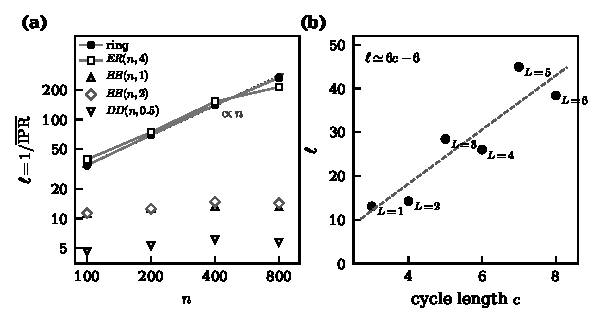
\includegraphics[width=\linewidth]{figs/fig-qw-scaling.pdf}
\caption{\textbf{Localized and delocalized.} (a) The localization volume
$\ell=1/\overline{\mathrm{IPR}}$ against size. The ring and the random network
(lines) grow in proportion to $n$, the dotted line showing that slope; the local
rules (markers) flatten, which is what localization means. (b) For the bubble family
$BB(n,L)$ at $n=800$, $\ell$ against the length $c=L+2$ of the cycle the rule
closes. The dashed line is a least-squares fit. The walker's territory is the size
of the rule's own footprint.}
\label{fig:qw-scaling}
\end{figure}

\section{It is not the clustering}
\label{sec:qw-clustering}

The natural reading of those numbers is the one
\citet{boettcher2025localization} give: these rules make triangles, triangles make
cliquish neighborhoods, and a cliquish neighborhood is a box the walker cannot get
out of. The table refutes it in a single comparison, and the comparison is available
only because Chapter~\ref{ch:bubbles} built the family that makes it.

$BB(n,1)$ and $BB(n,2)$ are the same rule. Both lay a chain of $L$ new nodes across
a randomly chosen link; the only difference is the length of the chain, $L=1$ or
$L=2$, and therefore the length of the cycle it closes, a triangle or a square.
$BB(n,1)$ has a mean clustering coefficient of $0.74$. $BB(n,2)$ has, exactly and by
construction, none at all: it is bipartite, and a bipartite network contains no
triangle whatsoever. Their localization volumes are the same, $13$ and $14$ at
$n=800$.

Zero triangles, identical trapping. Whatever confines the walker on $BB(n,1)$ is
still there when the triangles are removed, so it was never the triangles.

The wider view (Figure~\ref{fig:qw-tests}a) says the same less sharply but more
completely: across the rules of this book, $\ell$ and $\langle c\rangle$ are simply
unrelated. Rules with $\langle c\rangle$ identically zero span the entire range of
localization, from $DD(n,0.5)$ at $\ell\approx6$ --- the most tightly confined
random rule in the table --- to the ring, which is not confined at all. Rules with high
clustering are scattered through the middle. There is no monotone relationship to
find, and no amount of clustering is either necessary or sufficient.

Why, then, did clustering look like the answer? Because
\citet{boettcher2025localization} varied it in constructions where it was
confounded. Their recursive triangle web, the pseudofractal, Holme--Kim and the
Kleinberg model all raise clustering by \emph{adding short cycles}, and one cannot
add a triangle without also adding the shortest cycle there is. Turning up the
clustering knob in all four of their models turns up something else at the same
time, and Section~\ref{sec:qw-footprint} argues it is the something else that
matters. Their own numbers already order themselves that way: reading their figures
against the cycles their rules close rather than against clustering reproduces the
ranking of their curves.

\section{It is not the communities either}
\label{sec:qw-communities}

The next hypothesis is more attractive, and it is the one this book invites. The
localization volume is a number of nodes; communities are groups of nodes; and
Chapter~\ref{ch:graphons} showed that the rules here have a constant \emph{density}
of communities, so that mean community size $\langle n_B\rangle$ is a
size-independent number each rule owns --- exactly the sort of thing a
size-independent $\ell$ might be. On this reading the walker is confined to the
community it was born in, held there by the same faint seam that lets a block model
find the partition at all: Chapter~\ref{ch:communities} proved that the diamond's
boundary decays relative to its interiors like
$\lambda_{\mathrm{seam}}/\lambda_{\mathrm{vol}}=1/s$, and a boundary that fades is a
barrier the walker cannot tunnel through.

It is a good hypothesis. It is wrong, and the instrument that refutes it is again
one the book already built.

Chapter~\ref{ch:bubbles} needed two controls that closed the same square as
$BB(n,2)$ but differed in whether the resulting network had communities: $BB(n,2)$
itself has \emph{no communities at any size}, while adding one further link per step
--- either a link to a neighbor of the far endpoint, which keeps the network
bipartite, or the square's own diagonal, which does not --- puts both variants into
the constant-density class. Same rule, same motif, community structure switched on
and off. Figure~\ref{fig:qw-tests}b walks on all three.

The rule with no communities is the \emph{most strongly} localized of the three:
$\ell=14$ at $n=800$, against $34$ for the variant that adds a link and $16$ for the
one that adds a diagonal. All three sit at the same mean degree, $4.0$, so there is
nothing to blame on density. If communities were the trap, the network with none
could not be the one that traps hardest.

The quantitative check fails too. Across the whole table, $\ell$ never comes close to
$\langle n_B\rangle$ --- it is two to twelve times smaller everywhere --- and the two
do not even agree on the ordering: $BB(n,4)$ has the largest mean community of any
rule measured, $\langle n_B\rangle=304$, and a localization volume of $26$, smaller
than $BB(n,5)$'s $45$ at $\langle n_B\rangle=271$. The walker is not confined to a
community. It is confined to something several times smaller, and to something the
block model is not looking at.

And yet the failure has a shape, and it is a shape the book has already explained.
Look at \emph{which} rule the community hypothesis got wrong. $BB(n,2)$ reports no
communities because Chapter~\ref{ch:motifs} showed that an alphabet containing the
square books its structure as planted motifs instead --- and
Chapter~\ref{ch:bubbles} then showed that this is not a network changing but a
description changing dialect. The meso-structure did not go anywhere; it was
renamed. A rule whose footprint tiles the network cleanly spends its whole
meso-structure budget on motifs and reports no communities; a rule whose footprint
overlaps itself has a remainder, and the remainder is what gets bought at the
bespoke rate and counted as a community. What does not move, across the parity
alternation that sends $\kappa$ from $n^{0.25}$ to $n^{0.93}$, is the total
$\kappa_0+\kappa$.

If that is right, then the community hypothesis was not so much wrong as quoted in
the wrong currency. The walker is not doing inference and cannot see which dialect a
statistician chose; it responds to what is physically there. So it should be
measuring the invariant --- the meso-structure --- and not the residue that the
vocabulary happens to leave in community form. The next two sections test that, and
it is the reading that survives.

\begin{figure}[t]
\centering
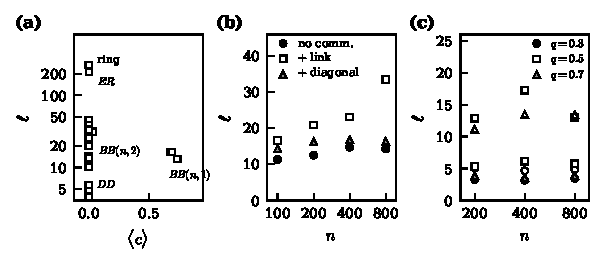
\includegraphics[width=\linewidth]{figs/fig-qw-tests.pdf}
\caption{\textbf{Three tests, two negative.} (a) $\ell$ against mean clustering at
$n=800$, one point per rule: no relationship. $BB(n,1)$ and $BB(n,2)$ are the same
rule at chain length $1$ and $2$ and localize identically, though one is built of
triangles and the other contains none. (b) The same square-closing rule with its
community structure switched on: $BB(n,2)$ has no communities at any size, the two
variants have a constant density of them, and the one with none localizes hardest.
(c) Duplication--divergence with and without its exact symmetries: filled markers as
grown, hollow markers with each class of identical-neighborhood twins collapsed to
one representative. The more of the network is exactly symmetric, the more of the
trapping is destroyed by removing the symmetry.}
\label{fig:qw-tests}
\end{figure}

\section{The volume is the footprint}
\label{sec:qw-footprint}

Return to the bubble family and read it as a family. $BB(n,L)$ closes a cycle of
length $c=L+2$, and $L$ is a dial that changes nothing else about the rule: the same
random link is chosen, the same chain is laid across it, only longer. Turning that
dial moves the localization volume, and moves it in the one way that makes sense
(Figure~\ref{fig:qw-scaling}b). A triangle-closing rule confines the walker to
about a dozen nodes. A rule closing a seven-cycle confines it to about forty-five.
The relation across the family is linear in the cycle length,
\begin{equation}
  \ell \;\simeq\; 6c - 6 ,
  \label{eq:qw-footprint}
\end{equation}
with the parity zig-zag familiar from Chapter~\ref{ch:bubbles} riding on top of it.

So the walker's territory is set by the size of the structure the rule keeps
building. Not by how cliquish that structure is --- the $c=3$ and $c=4$ members
differ by everything in clustering and by nothing in $\ell$ --- and not by how the
structures group themselves into communities, but by the plain linear size of the
rule's own footprint.

One confound has to be cleared before that reading is safe, because within the bubble
family the footprint is not quite the only thing $L$ changes. A step of $BB(n,L)$ adds
$L$ nodes and $L+1$ links, so the mean degree is $\langle k\rangle = 2(L+1)/L$ and
falls as the cycle lengthens, from $4$ at $L=1$ to $2.3$ at $L=6$. Longer footprints
therefore come with sparser networks, and one could ask whether
Eq.~\eqref{eq:qw-footprint} is a statement about cycles or merely about density.

It is about cycles, and the table settles it because several of its rows sit at
\emph{identical} mean degree. $BB(n,1)$, both $BB(n,2)$ variants, $LS(n,1)$ and
$BA(n,2)$ all have $\langle k\rangle=4.0$ to the precision quoted, and their
localization volumes run from $13$ to $34$ --- a spread of two and a half, at fixed
density. In the other direction, $BB(n,2)$ and the $(2,2)$ diamond both have
$\langle k\rangle\approx3.0$ and differ in $\ell$ by a factor of three. Density
matters, as it must, since a walker on a sparser network has fewer directions to go;
but it does not order these rules, and it cannot account for either of those spreads.

The deterministic lattices then confirm the reading with a second, independent dial,
and they matter because the diamond is the one construction in this book whose
community structure is known exactly rather than fitted.

\begin{center}
\footnotesize\setlength{\tabcolsep}{5pt}
\begin{tabular}{lrrrr}
\hline
lattice & $n$ & $\langle c\rangle$ & $\ell$ & $\ell_{\min}$\\
\hline
pseudofractal & $42$ & $0.78$ & $4.2$ & $3.2$\\
 & $123$ & $0.79$ & $3.8$ & $2.5$\\
 & $366$ & $0.80$ & $3.6$ & $2.3$\\
recursive triangle & $48$ & $0.78$ & $6.9$ & $2.7$\\
 & $96$ & $0.78$ & $7.9$ & $3.3$\\
 & $192$ & $0.78$ & $10.5$ & $3.8$\\
 & $384$ & $0.78$ & $12.3$ & $3.2$\\
diamond $(b,s)=(2,2)$ & $44$ & $0.00$ & $4.1$ & $3.4$\\
 & $172$ & $0.00$ & $4.3$ & $3.5$\\
 & $684$ & $0.00$ & $4.2$ & $3.5$\\
diamond $(2,3)$ & $30$ & $0.00$ & $5.9$ & $5.5$\\
 & $174$ & $0.00$ & $7.7$ & $6.4$\\
 & $1038$ & $0.00$ & $7.6$ & $6.4$\\
diamond $(2,4)$ & $56$ & $0.00$ & $8.7$ & $7.8$\\
 & $440$ & $0.00$ & $11.0$ & $9.1$\\
diamond $(3,2)$ & $23$ & $0.00$ & $2.5$ & $2.2$\\
 & $131$ & $0.00$ & $2.6$ & $2.2$\\
 & $779$ & $0.00$ & $2.5$ & $2.2$\\
diamond $(4,2)$ & $38$ & $0.00$ & $2.0$ & $1.8$\\
 & $294$ & $0.00$ & $2.0$ & $1.7$\\
\hline
\end{tabular}
\end{center}


The $(b,s)$ diamond replaces every link by $b$ parallel paths of $s$ links, and
Chapter~\ref{ch:communities} showed that the two parameters do quite different jobs:
$b$ sets how many communities there are, $s$ sets how sharply they separate, through
$\lambda_{\mathrm{seam}}/\lambda_{\mathrm{vol}}=1/s$. If the trap were the community
seam, $s$ would be the parameter that matters and larger $s$ --- a fainter seam ---
would mean tighter confinement. It is exactly backwards. Raising $s$ from $2$ to $3$
to $4$ at fixed $b$ \emph{loosens} the trap, from $\ell=4.2$ to $7.6$ to $11.0$,
because $s$ is also the length of the path the walker has to run along inside the
cell. Raising $b$ tightens it --- $4.2$, $2.5$, $2.0$ at $b=2,3,4$ --- because $b$ is
how many ways the cell branches at each junction, and this happens at essentially
fixed mean degree, $3.0$ to $3.4$ across the three. Both readings are geometric.
Neither is about the partition.

And every one of these numbers is flat in size, this time without qualification. The
$(2,2)$ diamond gives $\ell=4.1$ at $44$ nodes and $4.2$ at $684$; the $(2,3)$
diamond gives $7.7$ at $174$ nodes and $7.6$ at $1038$; the $(3,2)$ diamond gives
$2.5$ at $23$ nodes and $2.5$ at $779$. The lattices are the cleanest demonstration
available that $\ell$ is a property of the \emph{rule} rather than of the network the
rule happens to have produced so far, because for a lattice there is only one network
per size and the flatness cannot be an artifact of averaging over an ensemble.

The pseudofractal is the extreme case and it closes the loop with
\citet{boettcher2025localization}. Built entirely of triangles, the shortest cycle
there is, it confines the walker to $3.6$ nodes at $366$ --- the tightest trap of any
triangle rule in this book, and falling, not rising, with size.

Their own recursive triangle web behaves quite differently, and the difference is the
sharpest thing this chapter has to say about their paper. Its mean $\ell$ does not
settle and does not creep: it grows as a power, $\nu=0.46\pm0.05$ over $48$ to $1536$
nodes, close to $\sqrt{n}$ and unmistakably not a constant
(Section~\ref{sec:qw-exponent}). By the criterion of this chapter the average walker
on that lattice is not localized at all.

What is localized is a minority of starting points. The \emph{minimum} over start
nodes, $\ell_{\min}=1/\max_j\overline{\mathrm{IPR}_j}$, sits at about three at every
depth: a few nodes stay pinned onto a handful forever while the rest grow steadily
freer as the lattice grows. That heterogeneity is not a discrepancy with
\citet{boettcher2025localization} --- it is their own Figure~2, where the absolute and
relative gaps between the largest and smallest long-time IPR both widen with depth and
the minimum IPR tends to zero while the maximum stays finite. The two measurements
agree completely, which is the check that this chapter's instrument is theirs.

Where the readings part is what the agreement licenses. They present the lattice as a
demonstration that clustering localizes quantum walks. What it demonstrates is that
clustering localizes \emph{some} walkers on it, on a lattice whose typical walker
spreads over an unboundedly growing territory --- while the pseudofractal, built of the
same triangles by a rule that tiles them without leftovers, localizes every walker on
it at $\nu=-0.04$. Two triangle lattices, opposite verdicts. The triangle is not what
is doing the work.

What does not follow is their conclusion. Their flagship example is the extremum of
the footprint law, not the generic case: they found the tightest trap available
because the triangle is the shortest cycle there is, and then read the choice of
example as a mechanism.

\section{Measured in meso-units}
\label{sec:qw-meso}

The footprint law and Chapter~\ref{ch:bubbles} are two statements about the same
thing, and putting them side by side turns the chapter's negative results into a
positive one.

Chapter~\ref{ch:bubbles} measured, for the bubble family, the density of
meso-structure $b_0 = (\kappa_0+\kappa)/n$ --- motifs plus communities per node,
counted without regard to which vocabulary named them --- and found it to be a
constant of the rule that falls as the motif grows, from $0.38$ per node at $L=1$ to
$0.09$ at $L=5$, simply because a longer cycle uses more links per copy and fewer
copies fit. Its reciprocal $1/b_0$ is therefore the mean size of a meso-unit in
nodes: about $2.6$ nodes at $L=1$, rising to about $11$ at $L=5$.

Now measure the walker's territory in those units instead of in nodes.

\begin{center}
\footnotesize\setlength{\tabcolsep}{5pt}
\begin{tabular}{lrrrr}
\hline
rule & $c$ & $b_0$ & $\ell$ & $\ell\,b_0$\\
\hline
$BB(n,1)$ & $3$ & $0.38$ & $13$ & $5.0$\\
$BB(n,2)$ & $4$ & $0.20$ & $14$ & $2.8$\\
$BB(n,3)$ & $5$ & $0.15$ & $28$ & $4.3$\\
$BB(n,4)$ & $6$ & $0.12$ & $26$ & $3.1$\\
$BB(n,5)$ & $7$ & $0.09$ & $45$ & $4.0$\\
\hline
\end{tabular}
\end{center}


\noindent Across the family $\ell$ itself varies by a factor of three, from about a
dozen nodes to about forty-five, and it varies for the reason
Section~\ref{sec:qw-footprint} gave: the cell is getting bigger. But the walker's
territory measured in \emph{meso-units},
\begin{equation}
  \ell_0 \;=\; \ell\,b_0 ,
  \label{eq:qw-ell0-def}
\end{equation}
barely moves. It is a handful --- between $2.8$ and $5.0$ --- for every rule in the
family, with the same parity alternation riding on it that Chapter~\ref{ch:bubbles}
found in everything else (odd $L$ near $4.4$, even $L$ near $3.0$), and with no trend
in $L$ at all. Where $\ell$ spans a factor of $3.4$ across the family, $\ell_0$ spans
$1.7$, and within a parity class it is constant to a tenth.

That is the result the community hypothesis was reaching for and missing by one
change of units. The walker is confined to a few units of meso-structure. Whether a
statistician, handed the same network, would call those units motifs or communities
is a question about vocabulary that the walker cannot see and does not answer ---
which is exactly why $BB(n,2)$, whose meso-structure is booked entirely as motifs and
which therefore reports no communities at any size, sits on the same line as
$BB(n,3)$, whose meso-structure is booked largely as communities. Two dialects, one
substance, one localization volume per unit of it.

Read this way the chapter is an independent confirmation of Chapter~\ref{ch:bubbles}'s
central claim, arrived at by a route with no description length in it anywhere. That
chapter argued from minimum description length that a motif and a community are the
same object at two scales and that the invariant is their total. Here a quantum
walker, which knows nothing of priors or alphabets or block models, and which was put
on these networks to answer a different question entirely, agrees: it measures the
total, and it measures it in the units the total is denominated in.

\section{How localized, exactly?}
\label{sec:qw-exponent}

Section~\ref{sec:qw-flat} claimed that $\ell$ stops growing, and was careful to say
that the rules with the largest footprints had not visibly stopped by $n=800$. That
caution has to be paid for, because ``stops growing'' is a strong claim and the
obvious alternatives are hard to tell apart over three octaves of size. Three
candidates fit the same data:
\begin{equation}
  \ell \to \text{const}, \qquad
  \ell \sim a + b\ln n, \qquad
  \ell \sim n^{\nu}\ \ (0<\nu<1).
  \label{eq:qw-three}
\end{equation}
The first is localization. The third is something else entirely --- a walker whose
territory grows without bound but more slowly than the network, so that the
\emph{fraction} explored still vanishes. The second sits exactly between them.

The meso-unit picture of Section~\ref{sec:qw-meso} does not merely permit that
question; it answers it, and ties the answer to a number Chapter~\ref{ch:bubbles}
already measured.

\begin{calculation}{the localization exponent is one minus the census exponent}
Write $\ell_0$ for the walker's territory measured in meso-units rather than in nodes
--- the quantity Section~\ref{sec:qw-meso} tabulated as $\ell\,b_0$ --- so that by
definition
\begin{equation}
  \ell = \frac{\ell_0}{b_0}, \qquad b_0 = \frac{\kappa_0+\kappa}{n},
  \label{eq:qw-ell0}
\end{equation}
$b_0$ being the density of meso-structure. Chapter~\ref{ch:graphons} writes the
census as a power of the size and Chapter~\ref{ch:bubbles} measures it for the total,
$\kappa_0+\kappa \sim n^{\beta}$, whence $b_0\sim n^{\beta-1}$. If $\ell_0$ is a
constant of the rule --- which is what Section~\ref{sec:qw-meso} found, to within the
parity alternation --- then
\begin{equation}
  \ell \;\sim\; n^{\,1-\beta}, \qquad\text{that is}\qquad
  \boxed{\ \nu = 1-\beta\ }.
  \label{eq:qw-nu}
\end{equation}
The three cases of Eq.~\eqref{eq:qw-three} are therefore not three hypotheses about
quantum walks. They are the three limit classes of Chapter~\ref{ch:motifs}, read in a
different variable:
\begin{itemize}
  \item $\beta=1$, a constant density of meso-structure, gives $\nu=0$ and a
    localized walker. Every rule in this book is here.
  \item $0<\beta<1$, the \emph{fractal} class --- definable, and empty in
    Chapter~\ref{ch:motifs} --- gives $0<\nu<1$ and a walker whose territory
    grows as a power.
  \item $\beta=1$ with a logarithmic correction, $\kappa_0+\kappa\sim n/\ln n$, gives
    the marginal $\ell\sim\ln n$.
\end{itemize}
Two warnings about Eq.~\eqref{eq:qw-nu}. It fixes the exponent and not the
prefactor: Section~\ref{sec:qw-meso} bounds $\ell_0$ only between about $3$ and $5$,
so the dictionary is good to a factor of $1.7$ in the amplitude. And it assumes
$\ell_0$ does not itself depend on size --- which is exactly the assumption the
logarithmic case violates, since at $\beta=1$ the power vanishes and $\ell$ inherits
whatever $\ell_0(n)$ does. A log, if there is one, comes from $\ell_0$ and not from
$\beta$.
\end{calculation}

Equation~\eqref{eq:qw-nu} turns a vague claim into a prediction with numbers in
it. Chapter~\ref{ch:bubbles}'s fitted $\beta$ for $\kappa_0+\kappa$ runs from $0.94$
to $1.21$ across the book's rules, so $\nu$ should sit at $0$ to within about
$\pm0.2$ for all of them, and at $0.00$ for the deterministic lattices, whose $\beta$
is exactly one.

Deciding this needs a longer lever arm than Section~\ref{sec:qw-flat} used, and one
correction to the method. A fixed averaging window is not safe at large size: a
ballistic walker on a ring of $3200$ nodes has not crossed it by $t=800$, so the
window truncates the delocalized reference and biases every exponent downward. The
measurements here therefore average over $t\in[2n,4n]$, a window that grows with the
system, and run to $n=3200$ for the stochastic rules and to a few thousand nodes for
the lattices. The three candidates of Eq.~\eqref{eq:qw-three} are then fitted to
$\ell(n)$ and compared by corrected Akaike information, which penalizes the two
two-parameter models for their extra freedom, so that ``constant'' has to be beaten
rather than merely tied.

\begin{center}
\footnotesize\setlength{\tabcolsep}{4pt}
\begin{tabular}{lrrrl}
\hline
rule & sizes & $\nu$ & $\Delta\mathrm{AIC}_c$ & best fit\\
\hline
ring & $100$--$3200$ & $0.99\pm0.00$ & $68.2$ & $n^{\nu}$\\
$ER(n,4)$ & $100$--$3200$ & $0.94\pm0.10$ & $5.3$ & $n^{\nu}$\\
$BA(n,2)$ & $100$--$3200$ & $-0.02\pm0.05$ & $4.8$ & constant\\
$BB(n,1)$ & $100$--$3200$ & $0.01\pm0.02$ & $4.8$ & constant\\
$BB(n,2)$ & $100$--$3200$ & $0.08\pm0.03$ & $0.0$ & $\ln n$\\
$BB(n,3)$ & $100$--$3200$ & $0.15\pm0.04$ & $1.3$ & $\ln n$\\
$BB(n,5)$ & $100$--$3200$ & $0.20\pm0.02$ & $5.0$ & $\ln n$\\
$BB(n,6)$ & $100$--$3200$ & $0.20\pm0.04$ & $2.7$ & $\ln n$\\
$LS(n,1)$ & $100$--$3200$ & $0.06\pm0.03$ & $0.6$ & constant\\
$DS(n,0.5)$ & $100$--$3200$ & $-0.04\pm0.05$ & $4.3$ & constant\\
$DD(n,0.5)$ & $100$--$3200$ & $-0.02\pm0.05$ & $4.8$ & constant\\
$BB(n,2)+$ a link & $100$--$3200$ & $0.30\pm0.05$ & $1.7$ & $n^{\nu}$\\
$BB(n,2)+$ a diagonal & $100$--$3200$ & $0.08\pm0.03$ & $0.5$ & $\ln n$\\
pseudofractal & $42$--$1095$ & $-0.04\pm0.02$ & $6.2$ & constant\\
rec.\ triangle & $48$--$1536$ & $0.46\pm0.05$ & $1.8$ & $n^{\nu}$\\
diamond $(2,2)$ & $44$--$2732$ & $-0.00\pm0.01$ & $12.0$ & constant\\
\hline
\end{tabular}
\end{center}


\noindent The answer is not one answer, and the split is the most interesting thing
in the chapter.

The two controls behave exactly as they must, which is the first thing to check: the
ring gives $\nu=0.99\pm0.00$ and the random network $0.94\pm0.10$, both choosing the
power law over a constant by a wide margin. Scaling the window mattered --- under the
fixed window of Section~\ref{sec:qw-flat} the random network read $0.83$, the
truncation biasing it down --- and with that fixed, delocalization is measured at the
value it should have.

\emph{Genuinely localized, $\nu=0$.} Seven rules choose a constant over both
alternatives, and choose it on an instrument built to punish a constant for being
simple. $BB(n,1)$ gives $0.01\pm0.02$; $LS(n,1)$, $0.06\pm0.03$; the two duplication
rules, $-0.04$ and $-0.02$; the pseudofractal, $-0.04\pm0.02$ over nearly five
octaves. The strongest is the $(2,2)$ diamond: $\nu=-0.000\pm0.008$ across $44$ to
$2732$ nodes --- six doublings --- with a constant beating both two-parameter models by
twelve units of corrected Akaike information. That is as clean as a null result gets,
and it comes from a lattice with no ensemble scatter to average away.

\emph{Logarithmic.} Four rules prefer $a+b\ln n$, and they are all the same kind of
rule: the bubble family at long cycles. $BB(n,5)$ runs $29$, $36$, $45$, $50$, $52$,
$60$ across the sweep, monotone, and $\ln n$ beats a constant by five units and beats
the power law too; $BB(n,6)$ and $BB(n,3)$ do the same less emphatically. Their
nominal exponents, $0.15$ to $0.20$, are what a log looks like when a power law is
fitted to it.

This is the loophole the calculation box flagged, and it is worth being plain that it
is a real effect and not noise. At $\beta=1$ the power vanishes and $\ell$ inherits
$\ell_0(n)$; a logarithm therefore says that the walker slowly \emph{acquires}
meso-units as the network grows, at a rate that would take a factor of a thousand in
size to double its territory. Eq.~\eqref{eq:qw-nu} survives it, because the leading
behavior is still $n^{1-\beta}$ with $\beta=1$; what it does not do is predict the
marginal correction, and the correction is there.

Why the long cycles and not the short ones? The bubble rules with long cycles are the
sparsest networks in the table --- $\langle k\rangle$ falls to $2.3$ at $L=6$ --- and
the sparsest are the ones whose footprints only barely overlap. A rule whose cells
interlock tightly gives the walker a hard wall; a rule whose cells are long thin loops
joined at single links gives it a slow leak. That is a plausible story and this
chapter does not test it, which makes it the most concrete thing the chapter leaves
open.

\emph{Unresolved.} Two rules read as power laws and should not be reported as such.
$BB(n,2)+$a link gives $\nu=0.30\pm0.05$, against the $-0.10$ that
Eq.~\eqref{eq:qw-nu} predicts from its measured $\beta=1.10$ --- but its sequence is
not monotone, falling from $31$ at $n=800$ to $29$ at $1600$ before jumping to $49$ at
$3200$, and the largest size carries only two realizations. The honest reading is that
this rule is not measured well enough, not that it is a counterexample. And the
recursive triangle web gives $\nu=0.46\pm0.05$, on which see below.

So the fractal class stays empty. Nothing in this book localizes a walker with a
genuine exponent $0<\nu<1$, which is what Eq.~\eqref{eq:qw-nu} predicts from the fact
that nothing in this book has $\beta<1$. The dictionary holds where it was derived to
hold. What it did not anticipate --- and what a measurement over three octaves could
not have seen --- is that the marginal case comes with a logarithm attached for the
rules with the loosest footprints.

\begin{figure}[t]
\centering
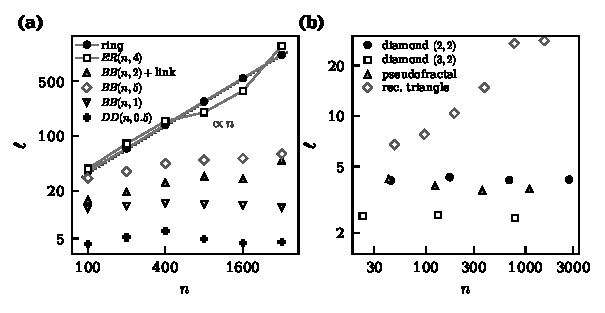
\includegraphics[width=\linewidth]{figs/fig-qw-exponent.pdf}
\caption{\textbf{What $\ell$ does over five octaves.} (a) Stochastic rules and the
two delocalized controls, with the averaging window scaled as $[2n,4n]$ and sizes to
$n=3200$; the dotted line is $\ell\propto n$. (b) The deterministic lattices, which
carry no ensemble scatter and so give the cleanest verdict: one network per size,
nothing averaged over.}
\label{fig:qw-exponent}
\end{figure}

\section{Duplication traps by symmetry}
\label{sec:qw-twins}

One rule in the master table is not explained by any of this, and it is the most
strongly localized of them all. Duplication--divergence, the gene-duplication rule
of Chapter~\ref{ch:duplication}, copies a node and then discards each copied link
with probability $q$. It closes no cycle of fixed length --- its motif is the
biclique $K_{2,d}$, the one motif in the book with no fixed size --- it has no
triangles, and it confines the walker to five nodes, tighter than any bubble rule.

The reason is the one the calculation box in Section~\ref{sec:qw-clustering}
anticipated: duplication does not merely make symmetric structure, it makes
\emph{exact} symmetry, and exact symmetry forces the eigenvalue degeneracies that a
large long-time IPR requires.

\begin{calculation}{why a duplicated node traps a walker}
Call two nodes $u$ and $v$ \emph{twins} if they are not adjacent and have identical
neighborhoods. A duplication step creates a twin outright, and divergence destroys
the relation only if it happens to delete a link, so at any moment a duplication
network carries many twin pairs. Twins have equal degree; call it $k$.

Consider the vector $x$ that is $+1/\sqrt{2k}$ on $u$, $-1/\sqrt{2k}$ on $v$, and
zero elsewhere, and apply $H=D^{-1/2}(D-A)D^{-1/2}$. At a node $i$ adjacent to both
twins,
\begin{equation}
  (Hx)_i = -\sum_j \frac{a_{ij}x_j}{\sqrt{k_ik_j}}
         = -\frac{x_u + x_v}{\sqrt{k_i\,k}} = 0 ,
  \label{eq:qw-twin-nb}
\end{equation}
the two contributions cancelling exactly because the amplitudes are equal and
opposite and the twins have the same degree. At every node adjacent to neither, all
terms vanish. And at $u$ itself the off-diagonal sum runs over $u$'s neighbors,
where $x$ is zero, leaving only the diagonal, so $(Hx)_u = x_u$; likewise at $v$.
Hence
\begin{equation}
  Hx = x ,
  \label{eq:qw-twin-eig}
\end{equation}
an eigenvector at eigenvalue exactly $1$, supported on two nodes, with
$\mathrm{IPR}=1/2$. A twin class of $c$ nodes contributes $c-1$ independent such
vectors, all at the same eigenvalue, so the degeneracy at $\lambda=1$ grows with the
amount of duplication. These are the terms of Eq.~\eqref{eq:qw-pibar} that survive
time-averaging, and they are maximally localized. A walker started on a twin is
partly frozen onto the pair forever.

Numerically the vector is exact --- $\|Hx-x\|$ vanishes to machine precision, and its
IPR is $0.5000$ --- but it accounts for only part of what is there. At $n=400$,
between $39\%$ and $55\%$ of the \emph{entire spectrum} of a $DD(n,q)$ network sits at
exactly $\lambda=1$, and the twins of Eq.~\eqref{eq:qw-twin-eig} force between a
quarter and seven tenths of that, the share rising with $q$. Duplication evidently
produces near-degenerate structure by routes beyond the twin relation --- pendant
nodes hanging off different parents will do it too --- so the theorem is a lower bound
on the degeneracy rather than an account of it. It is enough for the argument, since a
lower bound is all a mechanism needs.
\end{calculation}

Equation~\eqref{eq:qw-twin-eig} is elementary, but it has a consequence worth
spelling out: \emph{duplication localizes quantum walks by an exact theorem, with no
cycles and no clustering anywhere in the argument.} The trap is the symmetry itself.
Nothing about the network's global architecture enters, only the fact that two nodes
are interchangeable.

The prediction is testable by demolition. Take a grown $DD(n,q)$ network, find every
class of twins, and collapse each class to a single representative --- removing the
exact symmetries while leaving the rest of the architecture, the degrees, and the
overall size largely intact. If the twins are doing the trapping, the localization
should largely go away. Figure~\ref{fig:qw-tests}c does it, and the demolition works:
a quarter of the nodes of $DD(n,0.5)$ belong to a twin class, and merging them more
than doubles the localization volume at $n=800$, from $\ell=5.7$ to $13.0$, while the
most extreme confinement --- the walkers frozen with $\overline{\mathrm{IPR}}$ above
$0.7$, that is onto barely more than a single node --- is halved away, to $0.37$.

The strongest form of the test is the dose. Turn $q$, the probability that a copied
link is discarded, and the twin fraction moves with it, because a duplication that
loses no links leaves a perfect twin and one that loses many does not. At $q=0.3$,
$17\%$ of nodes are twinned and merging them costs the trap little, $\ell=3.4$ rising
to $4.8$. At $q=0.5$, $25\%$ are twinned and $\ell$ goes from $5.7$ to $13.0$. At
$q=0.7$, $43\%$ are twinned and $\ell$ goes from $3.9$ to $13.4$, a factor of three
and a half. The more of the network is exactly symmetric, the more of its trapping is
destroyed by removing the symmetry --- which is what a mechanism looks like, as
opposed to a correlation.

This also settles a detail of \citet{boettcher2025localization} that their
clustering account leaves unexplained. Following a walker on their recursive
triangle web, they observe that it ``predominantly alternates between two nodes.''
Two nodes is the signature of Eq.~\eqref{eq:qw-twin-eig}, and their lattice is full
of twins: every generation attaches new nodes across existing links, and two new
nodes laid across the same link are twins by construction. The two-node oscillation
they attribute to clustering is a symmetry, and it is the same symmetry that traps
walkers on protein interaction networks, where the duplication is real and the
triangles are not.

Whether real interactomes show it is a measurement this chapter does not make, and
it is the most concrete thing it leaves open. Duplicate genes are abundant and
long-lived \citep{ohno1970,force1999}, so the twins should be there; but real
divergence is not the independent link deletion of the model, and the question of how
long a twin survives in a genome is exactly the question of how quickly the symmetry
--- and therefore the trap --- decays.

\section{What the walker measures}

Put the three results together and the chapter has found a new kind of instrument.

The localization volume $\ell$ is size-independent, so it is a property of the rule
rather than of the sample. It is set by the footprint of the local rule --- the
length of the cycle closed, the branching of the cell, the exact symmetries a
duplication leaves behind --- and by nothing else the book measures. And it is
\emph{physical}: it is not a statistic computed by fitting a model but a number a
walker on the network produces by moving, and one already measured in the laboratory
on photonic chips \citep{tang2018}.

That last point is worth more than it first appears, because of a difficulty
Chapter~\ref{ch:communities} could not resolve. The Ramsey community number depends
on the method used to detect the communities, and the dependence is not small: on
one and the same network a plain block model and a degree-corrected one disagree by
a factor of twenty-five, and Chapter~\ref{ch:motifs} showed that changing only the
vocabulary can move a rule from having communities at $n=400$ to having none at any
size. A number that moves that much with the observer's choices is an awkward thing
to call a property of a network.

The localization volume has no such freedom. There is no prior to choose, no number
of blocks to infer, no alphabet to fix, no stochastic search that might not have
converged. One diagonalizes a matrix the network hands over and reads off a number.
Where Chapter~\ref{ch:communities} had to build its detection method into the
definition of what it was detecting, the walker just walks.

What it gives up is the partition. $\ell$ says nothing about \emph{which} nodes group
with which --- Section~\ref{sec:qw-communities} was the demonstration that it cannot
--- and it will not hand anyone a list of communities. But
Section~\ref{sec:qw-meso} showed that this is not the same as being blind to the
mesoscale. The walker sees the mesoscale; it simply sees the total rather than the
partition, and it sees the total in whichever dialect the network is actually built
in rather than the one a fit happened to choose. That is precisely the invariant
Chapter~\ref{ch:bubbles} had to reach for description length to isolate, and the two
routes to it could hardly be more different: one an argument about the cheapest way
to transmit a network, the other a wave packet failing to spread. Where they meet is
the best evidence in the book that the invariant is a thing and not an artifact of
how it was found.

There is a prediction in it, and it is easy to state and easy to falsify. If $\ell$
reads the footprint of a network's local rule, then real networks --- whose local
structure Chapter~\ref{ch:introduction} measured and Chapters~\ref{ch:friends}
to~\ref{ch:projects} accounted for --- should have localization volumes of a few
tens of nodes, independent of their size, and social networks built on triadic
closure should sit at the tight end of the range while networks whose local rule
closes longer cycles sit at the loose end. Sharper still: $\ell$ times the density of
meso-structure should come out at a few units, as it does for every rule here, and
Chapter~\ref{ch:graphons} has already measured the community side of that density
across some eighty real networks. Nothing here does the measurement. It is the
obvious next step, the data are the same repositories Chapter~\ref{ch:communities}
used, and the answer would be a statement about the local rule of a real system
obtained without fitting a model to it at all.

\section{Summary}

A classical walker forgets where it started and so can tell us only a network's
degrees; a quantum walker never forgets, and what it remembers turns out to be the
rule that built the network. Measuring the long-time inverse participation ratio on
every growth rule in this book gives a clean dichotomy: on networks grown by a local
rule the walker explores a share of the network that vanishes as it grows, and on a
ring or a random network it does not. Pushed over five octaves of size the dichotomy
resolves into three cases rather than two. Triadic closure, both duplication rules,
the pseudofractal and the diamond genuinely saturate --- the diamond at
$\nu=-0.000\pm0.008$ over six doublings, a constant preferred by twelve units of
Akaike information. The bubble rules at long cycles instead creep on like $\ln n$: a
marginal, log-divergent territory rather than a fixed one. And no rule anywhere shows
a genuine exponent $0<\nu<1$, which is exactly what $\nu=1-\beta$ predicts from the
fact that no rule in this book has $\beta<1$ --- so the fractal limit class of
Chapter~\ref{ch:motifs} is empty on this instrument too. The confinement is not caused by
clustering --- the same rule with its chain length changed from one to two has no
triangles at all and traps just as tightly --- and it is not caused by communities
--- the one square-closing variant with no communities at any size traps hardest of
the three. What sets the localization volume is the linear size of the rule's own
footprint, growing like $6c-8$ in the length $c$ of the cycle closed, tightening
when a deterministic cell branches more and loosening when its paths run longer.
Duplication is a case apart and the sharpest of all: twins are exact automorphisms,
they force eigenvectors of the walk Hamiltonian supported on two nodes, and merging
them triples the walker's territory. The pseudofractal and the recursive triangle
webs that provoked this chapter are then not evidence that clustering localizes
walks; they are the extreme point of the footprint law, the tightest trap available
because the triangle is the shortest cycle there is.

The community hypothesis, in the end, was right about the substance and wrong about
the units. Change the units --- count the walker's territory in the meso-structure of
Chapter~\ref{ch:bubbles} rather than in nodes --- and a localization volume that
varies threefold across the bubble family becomes the same handful of meso-units for
every rule in it, whether the description that network prefers spends its
meso-structure on motifs or on communities. What the walker measures is that
invariant: physically, with no model to fit, no alphabet to fix, and no partition to
infer.
